\documentclass[12pt,a4paper]{article}

\usepackage[utf8]{inputenc}
\usepackage[T5]{fontenc}
\usepackage[vietnamese]{babel}
\usepackage{geometry}
\usepackage{graphicx}
\usepackage{booktabs}
\usepackage{float}
\usepackage{array}
\usepackage{longtable}
\usepackage[hidelinks]{hyperref}

\geometry{left=3cm,right=2cm,top=2cm,bottom=2cm}

\title{BÁO CÁO BÀI TẬP LỚN\\
ĐỀ TÀI 9: DỰ ĐOÁN KHÁCH HÀNG RỜI BỎ DỊCH VỤ VIỄN THÔNG}
\author{Nhóm: Hùng (Đội trưởng), Mạnh, Đức, Hải}
\date{Năm học 2026--2027}

\begin{document}

\maketitle
\tableofcontents
\newpage

\section{Đặt vấn đề}
Khách hàng rời bỏ dịch vụ (customer churn) là bài toán phân loại nhằm dự đoán khả năng một khách hàng ngừng sử dụng dịch vụ viễn thông. Mục tiêu của đề tài là xây dựng và so sánh các mô hình học máy trên cùng tập kiểm tra để đánh giá khả năng nhận diện nhóm khách hàng có nguy cơ rời bỏ.

\section{Mô tả và khám phá dữ liệu}
% Hùng ghép phần EDA do Mạnh cung cấp vào đây.
\textit{Phần này sẽ được cập nhật từ kết quả EDA của Mạnh.}

\section{Tiền xử lý dữ liệu}
\subsection{Chia dữ liệu Train/Test}
Nhóm thống nhất chia dữ liệu bằng \texttt{train\_test\_split} với các tham số:
\begin{itemize}
    \item \texttt{test\_size = 0.20}
    \item \texttt{random\_state = 42}
    \item \texttt{stratify = y}
\end{itemize}
Việc cố định cách chia dữ liệu giúp các mô hình được đánh giá trên cùng một tập Test.

\subsection{Luồng A}
% Ghép mô tả tiền xử lý của Mạnh: missing value, One-Hot Encoding, StandardScaler.
\textit{Cập nhật nội dung Luồng A từ Mạnh.}

\subsection{Luồng B}
% Ghép Feature Engineering của Đức.
\textit{Cập nhật nội dung Luồng B từ Đức.}

\section{Thiết kế giải pháp}
\subsection{Decision Tree}
% Ghép mô tả thuật toán và GridSearchCV của Đức.
\textit{Cập nhật từ Đức.}

\subsection{K-Nearest Neighbors}
Thuật toán K-NN (K-Nearest Neighbors) dự đoán nhãn của mẫu mới dựa trên đa số phiếu bầu của $k$ láng giềng gần nhất trong không gian đặc trưng. Khoảng cách giữa các mẫu được đo bằng chuẩn khoảng cách Euclidean hoặc Manhattan:
\begin{itemize}
    \item Khoảng cách Euclidean: $d(x, y) = \sqrt{\sum_{i=1}^p (x_i - y_i)^2}$
    \item Khoảng cách Manhattan: $d(x, y) = \sum_{i=1}^p |x_i - y_i|$
\end{itemize}
Do K-NN hoàn toàn dựa trên khoảng cách hình học, dữ liệu đưa vào bắt buộc phải được chuẩn hóa về cùng thang đo để tránh các đặc trưng có biên độ lớn (như \texttt{MonthlyCharges} hay \texttt{tenure}) chi phối kết quả:
\begin{itemize}
    \item \textbf{Luồng A:} Sử dụng tập dữ liệu đã được tiền xử lý và chuẩn hóa tập trung trên toàn bộ tập Train từ khâu của Mạnh để đảm bảo tính đồng bộ giữa các thành viên.
    \item \textbf{Luồng B:} Được đóng gói hoàn chỉnh qua \texttt{Pipeline} kết hợp \texttt{StandardScaler} và \texttt{KNeighborsClassifier}. Quy trình chuẩn hóa diễn ra độc lập bên trong từng fold huấn luyện trong quá trình kiểm định chéo (5-fold Stratified CV), đảm bảo tính cô lập dữ liệu tuyệt đối và ngăn ngừa rò rỉ thống kê giữa các fold (fold-level leakage).
\end{itemize}
Không gian siêu tham số được tinh chỉnh gồm $k \in \{3, 5, 7, 9, 11, 15, 21, 31, 41, 51\}$, phương pháp gán trọng số \texttt{weights} (\texttt{uniform}, \texttt{distance}) và hệ đo khoảng cách (\texttt{euclidean}, \texttt{manhattan}), với mục tiêu tối ưu hóa chỉ số F1-score của lớp \texttt{Churn = Yes}.

\subsection{Chỉ số đánh giá}
Các mô hình được đánh giá bằng Accuracy, Precision, Recall, F1-score và Confusion Matrix. Đối với bài toán Churn, Recall và F1-score của lớp \texttt{Churn = Yes} được chú ý bên cạnh Accuracy vì lớp khách hàng rời bỏ có thể không chiếm đa số.

\section{Kết quả thực nghiệm}
Hùng tổng hợp bốn kết quả: Decision Tree trên Luồng A/B và K-NN trên Luồng A/B sau khi đánh giá trên cùng tập Test gồm 1.409 mẫu.

\begin{table}[H]
\centering
\small
\begin{tabular}{llcccc}
\toprule
Mô hình & Luồng & Accuracy & Precision & Recall & F1-score \\
\midrule
Decision Tree & A & 0.7488 & 0.5175 & \textbf{0.7914} & \textbf{0.6258} \\
Decision Tree & B & 0.7346 & 0.5000 & \textbf{0.7995} & 0.6152 \\
K-NN          & A & 0.7864 & 0.5968 & 0.6016 & 0.5992 \\
K-NN          & B & \textbf{0.7906} & \textbf{0.6238} & 0.5321 & 0.5743 \\
\bottomrule
\end{tabular}
\caption{Bảng so sánh chéo bốn kết quả mô hình trên tập Test chung.}
\label{tab:model-comparison}
\end{table}

\subsection{Ma trận nhầm lẫn}
Hình~\ref{fig:dt-cm} và Hình~\ref{fig:knn-cm} thể hiện ma trận nhầm lẫn của Decision Tree và K-NN trên cả hai luồng đặc trưng.

\begin{figure}[H]
\centering
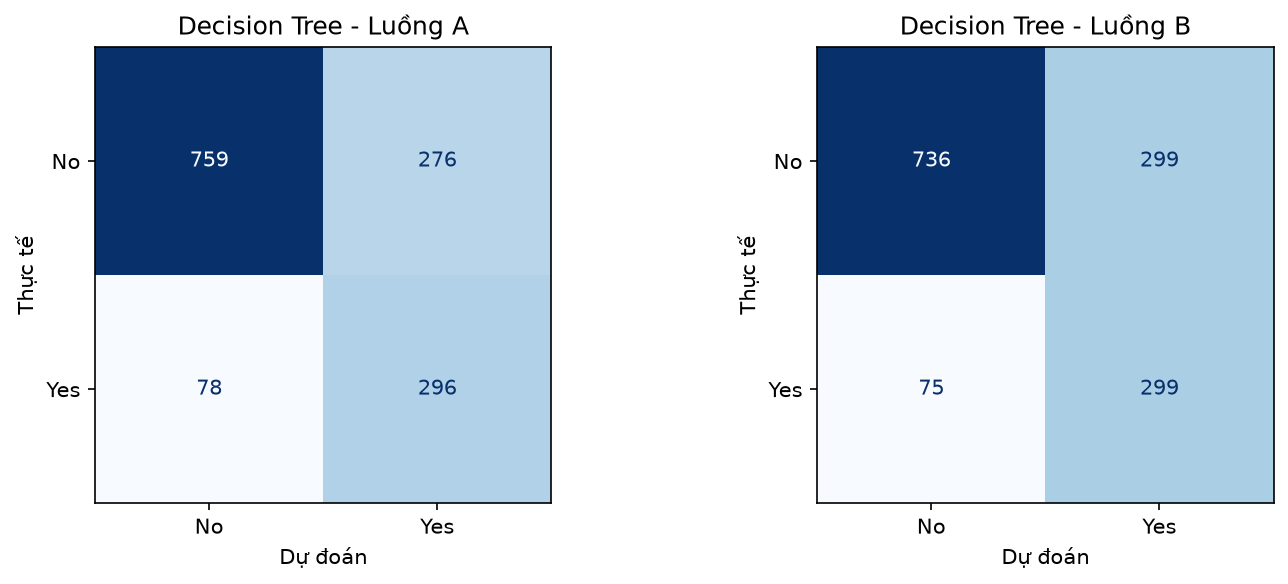
\includegraphics[width=0.85\textwidth]{figures/dt_confusion_matrix.png}
\caption{Ma trận nhầm lẫn của Decision Tree trên Luồng A và Luồng B.}
\label{fig:dt-cm}
\end{figure}

\begin{figure}[H]
\centering
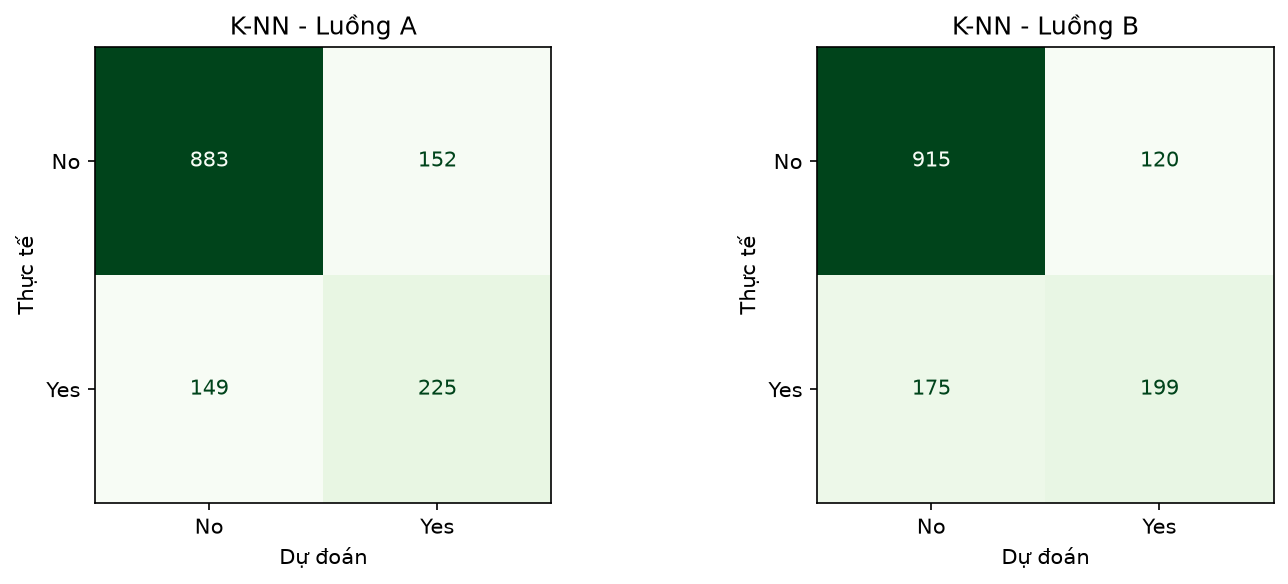
\includegraphics[width=0.85\textwidth]{figures/knn_confusion_matrix.png}
\caption{Ma trận nhầm lẫn của K-NN trên Luồng A và Luồng B.}
\label{fig:knn-cm}
\end{figure}

\section{Phân tích lỗi (Error Analysis)}
Dựa trên mô hình có F1-score tốt nhất là Decision Tree Luồng A (bắt được 296/374 khách hàng rời mạng, $F_1 = 0.6258$) và mô hình K-NN Luồng A ($F_1 = 0.5992$), nhóm tiến hành phân tích các trường hợp dự đoán sai trên tập Test chung:

\begin{figure}[H]
\centering
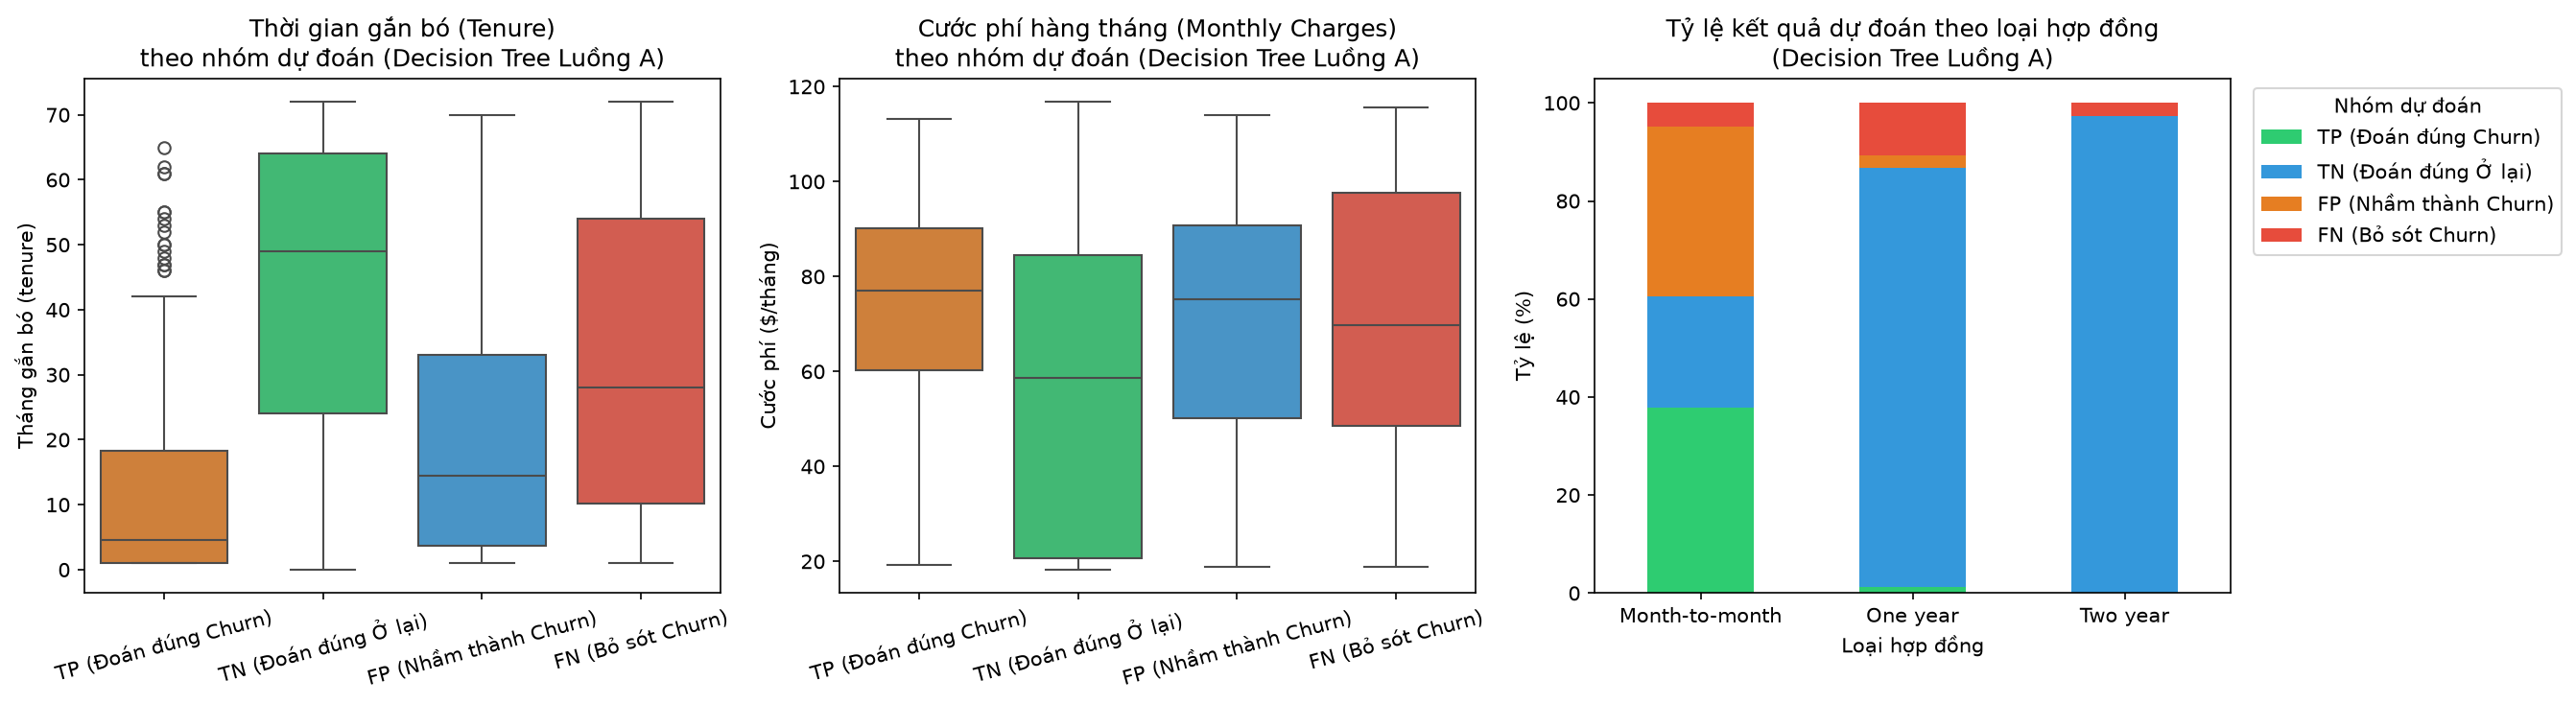
\includegraphics[width=0.95\textwidth]{figures/error_analysis_decision_tree.png}
\caption{Phân tích phân bố các nhóm dự đoán của Decision Tree Luồng A.}
\label{fig:error-dt}
\end{figure}

\begin{itemize}
    \item \textbf{False Negatives (Bỏ sót khách Churn - Nguy hiểm nhất):}
    Decision Tree chỉ bỏ sót 78 khách hàng (5.5\% tập Test), trong khi K-NN bỏ sót tới 149 khách hàng (10.6\%). Khảo sát sâu nhóm khách hàng FN cho thấy thời gian gắn bó trung bình của họ cao hơn hẳn nhóm Churn thông thường (31.7 tháng so với 12.4 tháng của nhóm TP), và có tới hơn 52\% khách hàng FN sở hữu hợp đồng dài hạn (1 năm hoặc 2 năm). Do mô hình học được quy luật thống kê chung là ``khách hàng hợp đồng dài hạn và thâm niên lâu có xác suất rời mạng thấp'', nên mô hình có xu hướng phân loại nhầm nhóm này thành Ở lại. Về mặt kinh doanh, nhóm nghiên cứu đặt giả thuyết rằng các ca rời mạng này có thể xuất phát từ các yếu tố ngoại cảnh chưa được số hóa trong tập dữ liệu (ví dụ: thay đổi địa điểm sinh sống, sự cố gián đoạn dịch vụ cục bộ, hoặc các yếu tố cá nhân ngoài các trường thông tin hợp đồng hiện có).
    
    \item \textbf{False Positives (Nhầm khách ở lại thành Churn):}
    Decision Tree có 276 trường hợp FP (19.6\%), K-NN có 152 trường hợp FP (10.8\%). Khảo sát cho thấy hơn 97\% khách hàng FP sử dụng loại hợp đồng từng tháng (\texttt{Month-to-month}) và có mức cước phí hàng tháng khá cao ($\approx 70.8\$$/tháng). Vì hồ sơ sử dụng của họ mang đầy đủ đặc trưng định lượng của nhóm rủi ro cao, mô hình dự đoán họ sẽ Churn, nhưng trên thực tế họ vẫn chọn tiếp tục sử dụng. Nhóm này là đối tượng phù hợp để nhà mạng triển khai các chính sách chăm sóc, tri ân giảm cước nhằm chuyển hóa sang hợp đồng dài hạn.
\end{itemize}

\section{Thảo luận}
Từ bảng so sánh thực nghiệm và phân tích lỗi, nhóm rút ra các nhận định then chốt:
\begin{enumerate}
    \item \textbf{So sánh giữa Decision Tree và K-NN:}
    \begin{itemize}
        \item K-NN đạt Accuracy tổng thể cao hơn ($\approx 79.1\%$) và Precision cao hơn ($\approx 62.4\%$), tuy nhiên Recall của lớp Churn chỉ đạt $53.2\% - 60.2\%$, tức là bỏ sót tới gần một nửa lượng khách hàng sắp rời mạng. Điều này là do K-NN đưa ra quyết định dựa trên số đông $k$ láng giềng gần nhất, mà trong tập dữ liệu Churn chỉ chiếm $26.5\%$, khiến ranh giới quyết định của K-NN có xu hướng thiên vị lớp đa số (\texttt{No}).
        \item Ngược lại, Decision Tree với kỹ thuật cân bằng trọng số (\texttt{class\_weight="balanced"}) đã ưu tiên phát hiện lớp thiểu số, đạt Recall vượt trội lên tới $79.1\% - 80.0\%$, bắt được gần $80\%$ khách hàng rời bỏ. Trong bài toán kinh doanh viễn thông, chi phí bỏ sót một khách hàng rời mạng (chi phí mất doanh thu dài hạn) lớn hơn nhiều so với chi phí gửi chương trình khuyến mãi nhầm cho khách hàng ở lại. Vì vậy, Decision Tree là mô hình có giá trị ứng dụng thực tiễn cao hơn.
    \end{itemize}

    \item \textbf{So sánh giữa Luồng A và Luồng B:}
    \begin{itemize}
        \item \textbf{Luồng A (45 đặc trưng):} Giữ lại toàn bộ thông tin chi tiết qua One-Hot Encoding, giúp Decision Tree đạt F1-score cao nhất ($0.6258$) và K-NN đạt F1-score $0.5992$.
        \item \textbf{Luồng B (17 đặc trưng):} Tinh gọn dữ liệu dựa trên hiểu biết nghiệp vụ (đặc trưng tương tác \texttt{MonthToMonth\_Fiber}, số dịch vụ bảo vệ còn thiếu \texttt{MissingProtectionCount}). Luồng B giúp giảm hơn $60\%$ số lượng chiều không gian nhưng vẫn duy trì độ chính xác và Recall tương đương (Recall Decision Tree Luồng B đạt tới $79.95\%$), mang lại tốc độ suy luận nhanh và khả năng giải thích trực quan cao hơn.
    \end{itemize}
\end{enumerate}

\section{Tổng kết}
Đề tài xây dựng một quy trình thống nhất từ chia dữ liệu, tiền xử lý, huấn luyện đến đánh giá mô hình. Bốn kết quả được kiểm tra trên cùng tập Test để đảm bảo việc so sánh công bằng. Phần tổng kết cuối cùng sẽ được cập nhật sau khi nhóm hoàn thành thực nghiệm và phân tích lỗi.

\end{document}
